\noindent \rule{0.75\linewidth}{0.3pt}
\section{Shafts and axles}

\begin{multicols} 2

	While dimensioning/verifying shaft it's important to use the \textbf{service factor}, a coefficient used to increment the nominal value in order to take into account possible torque overload in particular working condition; usually this coefficient is reported in table like in table \ref{tab:servicefactor}.
	
	\begin{table*}
	\centering
	\begin{tabular}{ r || M{3.5cm} | M{3.5cm} }
		& Normal torque & High torque and/or non uniform working \\ \hline
		Uniform functioning &  1.0-1-1 &  1.2-1-3 \\
		Light impact & 1.2-1.3 & 1.3-1.4 \\
		Moderate impact & 1.4-1.5 & 1.5-1.6 \\
		High impact & 1.5-1.6 & 1.6-1.8
	\end{tabular}
	\caption{service factor in respect of the characteristic of the driven machine.}
	\label{tab:servicefactor}
	\end{table*}	

	In general the design/verification process is firstly made for stress, then for the stiffness (excessive deflection that might lead to a non operating machine) and then for the critical flexural speed and torsional oscillations. In general while design a shaft we consider only the torsional and bending loading (they are most relevant in the shaft).
 	
 	\paragraph{Preliminary dimensioning} For a preliminary dimensioning of the shaft we can consider a full/hollow circle cross section that lead to a tension component $\tau$ equals
 	\begin{equation} \label{eq:shaft:torsion}
 		\tau = \frac{T}{J_p} \frac d 2
 	\end{equation}
 	where $T$ is the torque, $J_p$ is the torsional coefficient of the section (that for the circle cross section is equal to $\frac{\pi}{32}d^4$) and $d$ the diameter of the shaft. In order to take into account the bending load on the beam we can use a simplified approach to dimension the shaft considering an equivalent bending moment $M_{b,eq}$:
 	\begin{equation} \label{eq:shaft:bending}
 		M_{b,eq} = \sqrt{M_b^2 + \alpha T^2}
 	\end{equation}
 	where
 	\[ \alpha = \begin{cases}
 		0.25 \quad & T \textrm{ constant} \\
 		0.75 \quad & T \textrm{ alternating} \\
 	\end{cases} \]
	At this point we can compute the tension of the material $\sigma$ of the equivalent bending moment of the structure as
	\begin{equation}
		\sigma = \frac{M_{b,eq}}{Z}
	\end{equation}
	where $Z$ is the section modulus that, for the full circle cross section, is equal to $Z = \frac{\pi}{32} d^3$.
	
	In general the equivalent tension $\sigma_{eq}$ should be always less or equal to an allowable value $\sigma_{all}$; by inverting equations \ref{eq:shaft:torsion} and \ref{eq:shaft:bending} we can define the minimum diameter $d_{min}$ of a full circle cross section of the shaft that permits the correct holds of the loads:
	\begin{equation} \label{eq:shaft:dmin}
	\begin{split}
		d_{min} & \geq \sqrt[3]{\frac{32}{\pi} \frac{M_{b,eq}}{\sigma_{all}} } \quad \,\textrm{: bending,torsion} \\
		& \geq \sqrt[3]{\frac{16}{\pi} \frac{T}{\tau_{all}} } \qquad \textrm{: torsion} 
	\end{split}
	\end{equation}

	For the fatigue resistance allowable stress must be reduced using large safety factor. 
	
	For the selection of the material the most important parameter to consider is the yield strength because the material is responsible \textit{only} for the strength of the shaft, while the deflections and stresses can be handled by choosing a correct geometry for the section.
	
	\paragraph{Geometry definition} Known the minimum diameter on the shaft in order to support the loads applied, if we want to add some shoulder we have to keep in mind the following \textit{rules} in order to reduce the stress concentrations:
	\[ 1.2 \leq \frac D d \leq 1.5 \quad \textrm{and} \quad 0.02 \leq \frac r d\leq 0.06 \]
	where $D,d$ are respectively the diameters of the bigger and the smaller cross section of the shaft and $r$ is the fillet radius. At this stage it's important to use stress concentration factors $K_t$ that, for the design phase, can be computed considering the worst case scenario $D/d = 1.5$ and $r/d = 0.02$.

	While computing the stiffness verification always keep in mind that usually bearing have a maximum angle of deflection allowable: value above that limit might lead to a premature failure of the component. While computing deflection (using as example the Castigliano's theorem) it's not necessary to take into account stress concentration factors because they don't have an high \textit{impact} in terms of deflection.
	
	\subsection{Positive (geometric) coupling: parallel keys}
		Knowing the desirable torque $T$ to transmit from the shaft to a hub (using a parallel key) we can compute the pressure $p$ on the sides of the key assuming that the pressure is uniformly distributed:
		\[ p \simeq \frac{2T}{d(h-t) L} \]
		where $L$ is the key length and the other dimension as described in the next figure.
		\begin{center}
			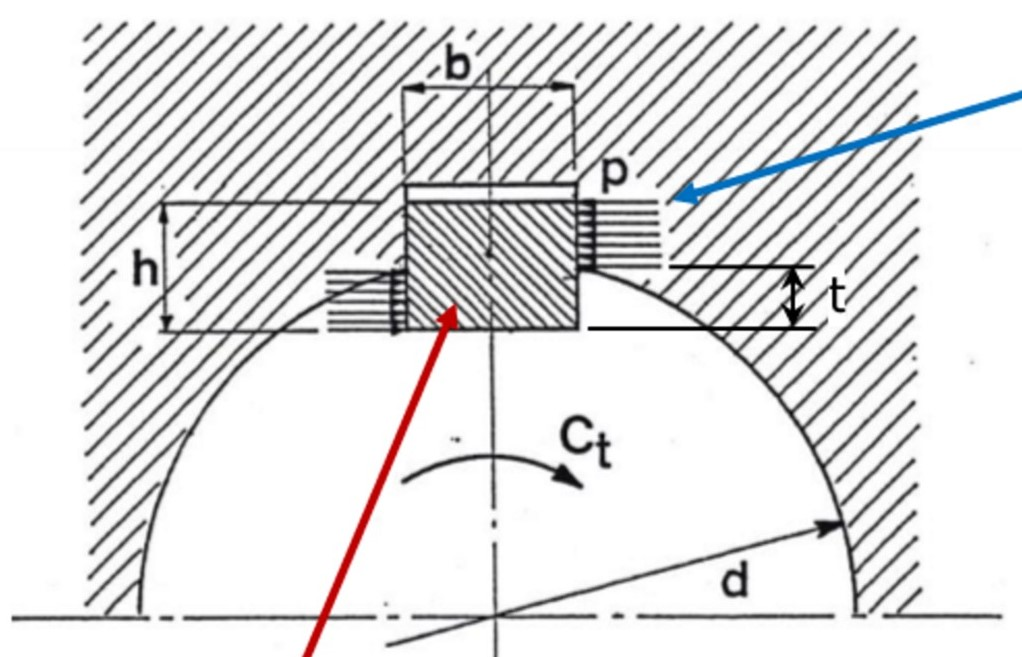
\includegraphics[width=4cm]{pos-coupling}
		\end{center}
		In reality the dimensioning of the keys is determined by normative (\texttt{UNI 6604}) where given the diameter $d$ of the shaft, all the other dimension are set (for example $b,h$), where only the length $L$ can be chosen insider a specific range (in order to adjust the pressure transmitted between the shaft and the gear). Good rule of thumb is that $L < 1.5d$. \\
		In order to transmit more pressure (and so torque) up to three key are allowed to be mounted on the shaft: in this case the pressure is determined as
		\[ p \simeq \frac{2T}{d(h-t)L z \phi} \]
		where $z$ is the number of keys and $\phi$ is the uniformity factor determined by the following table:
		\begin{center}
		\begin{tabular}{c|c}
			$z$ & $\phi$ \\ \hline 
			1 & 1 \\ 2 & 0.75 \\ 3 & 0.67
		\end{tabular}
		\end{center}
		While verifying pieces with keys inserted, new tables with stress concentration factors $K_t$ must be consider.
		
		\paragraph{Splines} Positive coupling with splines is ideal when the torque to be transmitted is high; in this case the major drawback is the introduction of high notch effects that worsen the response to fatigue.
		\begin{center}
			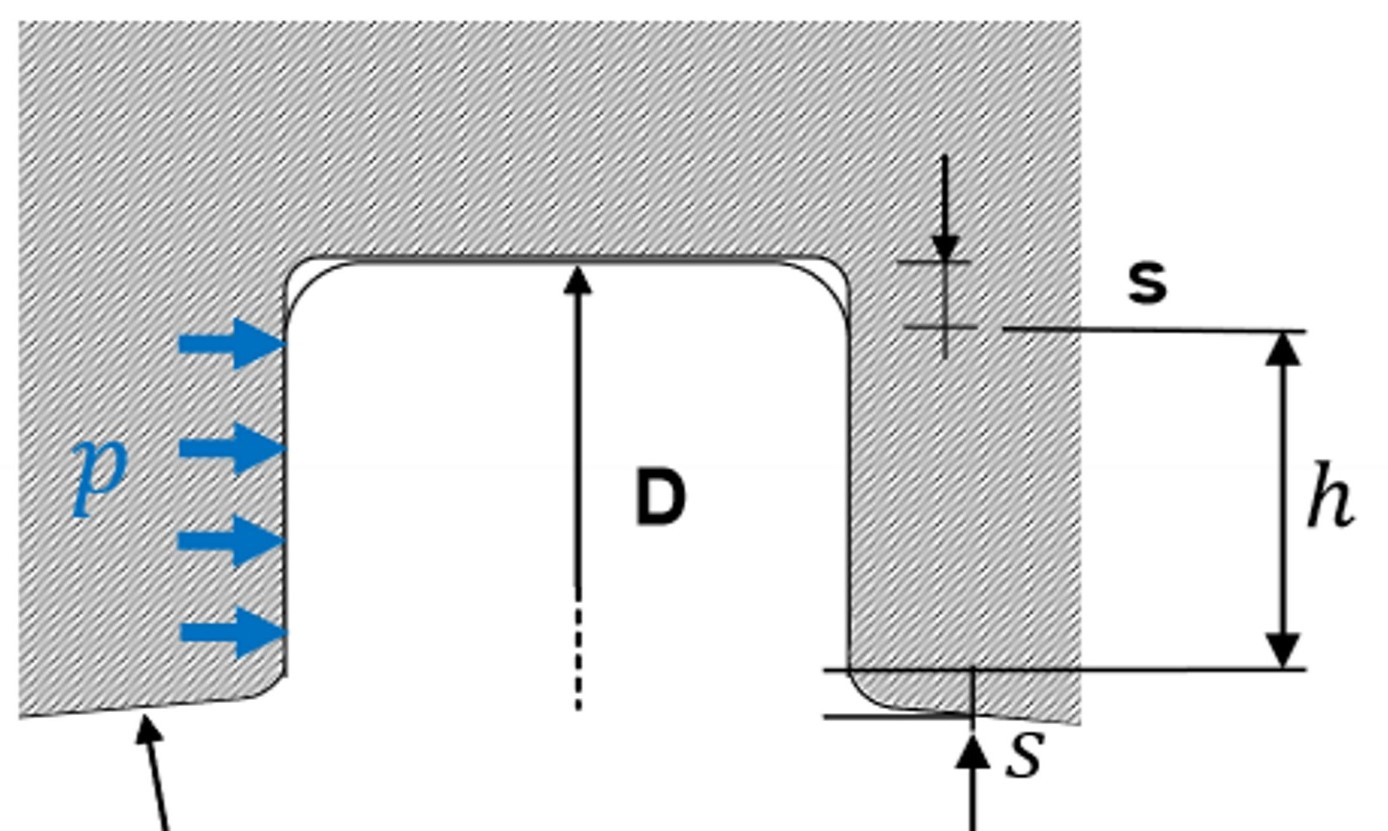
\includegraphics[width=4cm]{splines-dimensioning}
		\end{center}
		
		In order to dimension the spline we have to define the minimum shaft diameter in order to transmit the torque (equation \ref{eq:shaft:dmin}); the outer diameter $D$ related to the gear can be then calculated by looking at normative (\texttt{UNI 8953}) and last determine the length of engagement $L$ by imposing by making equally critical the shaft yielding and the spline profile bearing:
		\[ T_{max} = p_{all} h L \frac{d_m}{2} z \psi = \tau_{all,shaft} \frac{\pi d^3}{16} \]
		In this equation $d_m$ is the mean diameter computed as $\frac{D+d}{2}$, $z$ is the number of teeth and $\psi$ is a load distribution factor that's tabled (table \ref{tab:shaft:loaddistr}).
		
		\begin{table*}
		\centering
		\begin{tabular}{M{5cm}  || M {4cm} | M {4cm} }
			Contact surfaces & not sliding; sliding only when loaded & sliding when loaded \\ \hline
			both surfaces hardened & $\psi = 0.55$ & $\psi = 0.65$ \\
			no surfaces or one surface hardened & $\psi = 0.75$ & $\psi = 0.90$
		\end{tabular}
		\caption{load distribution factor $\psi$ function of load type and contact surfaces.}
		\label{tab:shaft:loaddistr}
		\end{table*}
	
	\subsection{Friction coupling: tapered press fits}
		In order to transmit torque using press fits the shaft has to present a conical section (that's complementary to the one on the hub that have to be installed on top of it) defined by the conicity ratio
		\[ C= \frac{D-d}{L} = 2 \tan \left(\frac \alpha 2\right)\]
		\begin{center}
			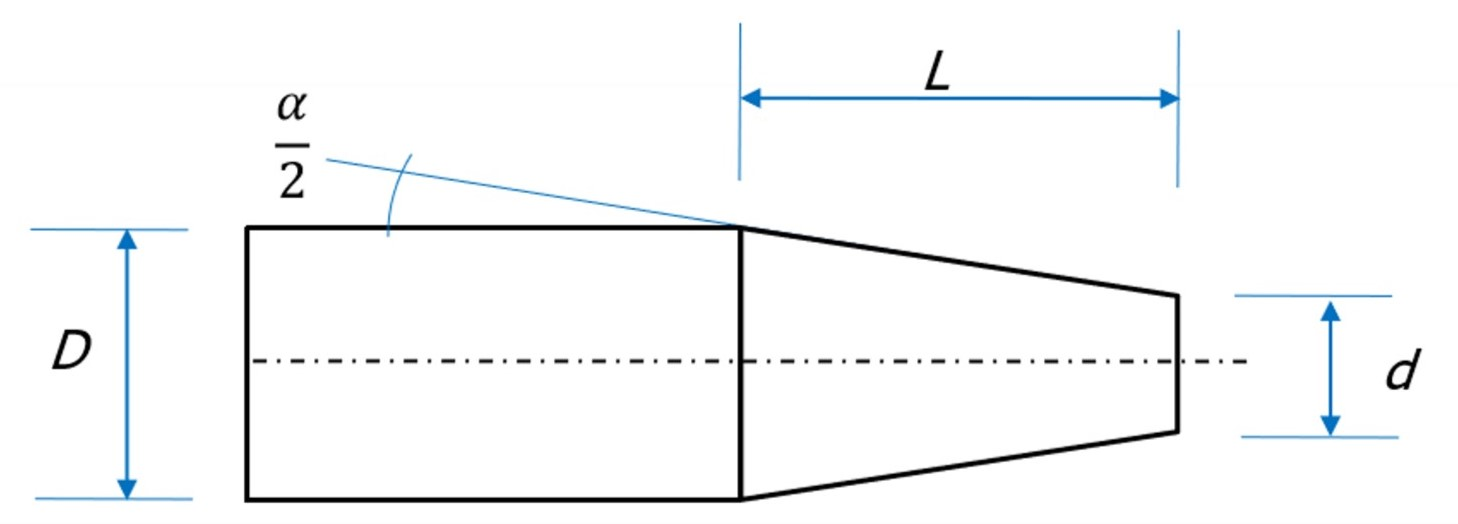
\includegraphics[width=0.9\linewidth]{pressfit-1}
		\end{center}
	
		By analysing the contact forces between the shaft and the hub it's possible to compute the minimum pressure on the contact $p_{min}$ (that should be always smaller than an allowable pressure $p_{all}$) and the torque $T$ transmitted as function of the axial force $F_a$, the axial ($f_a$) and torsional ($f_t$) friction coefficients:
		\begin{equation}
		\begin{split}
			p_{min} & = \frac 4 \pi \frac{F_a \sin(\alpha/2)}{D^2-d^2} \left( \frac 1 {\sin(\alpha/2) + f_a\cos(\alpha/2)} \right) \\
			T & = \frac 1 3 \left( \frac{f_t F_a}{\sin(\alpha/2) + f_a\cos(\alpha/2)} \right) \frac{D^3-d^3}{D^2-d^2}
		\end{split}
		\end{equation}
	
		\begin{center}
			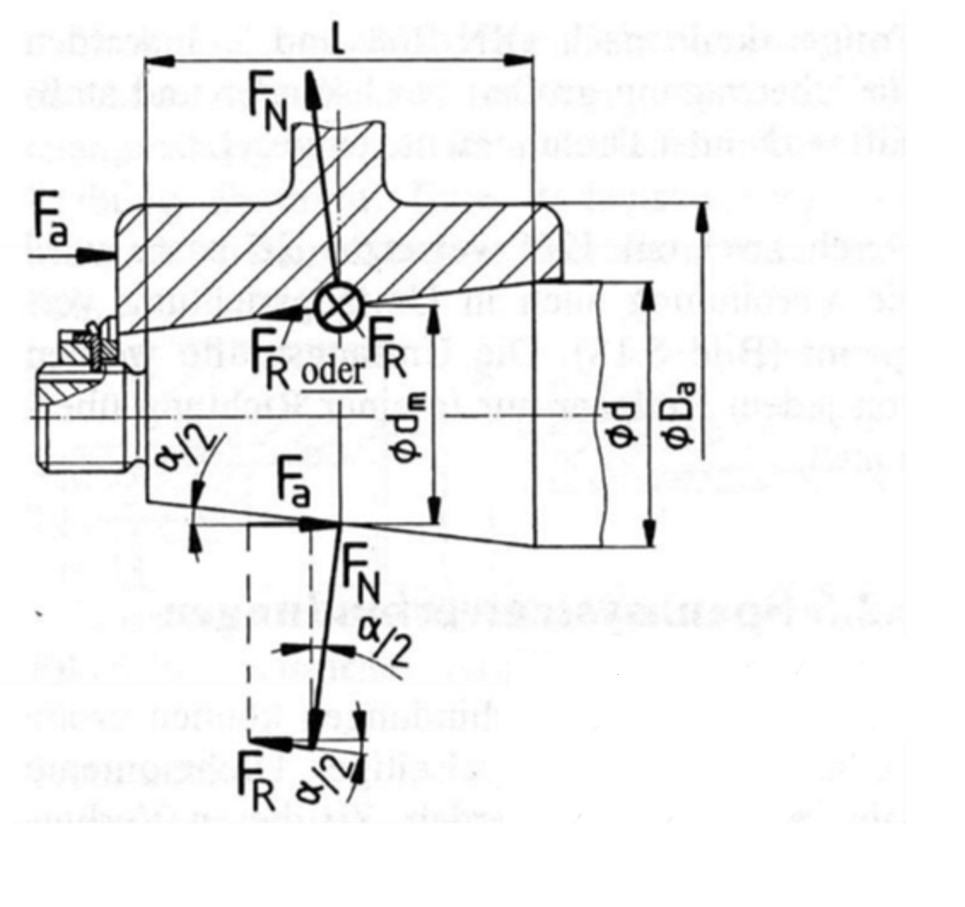
\includegraphics[width=5cm]{pressfit-2}
		\end{center}
		
		\paragraph{Press (interference) fit considerations} The interference $i$ between the dimensions of the outer radius $r$ of the shaft and the inner radius $R$ of the hub has to have a minimum value $i_{min}$ in order to avoid slipping between the two pieces, but also a maximum value $i_{max}$ in order to avoid yielding.
		
		In particular, by doing a full analysis, we can see that the interference $i$ is linearly proportional to the pressure $p_c$ happening on the surfaces in contact:
		\[ i = p_c r_c \left( \frac 1 {E_2} \frac{R^2+r_c^2}{R^2-r_c^2} + \frac{\nu_2}{E_2} + \frac{1}{E_1}  \frac{r_c^2 + r^2}{r_c^2 - r^2} - \frac{\nu_1}{E_1}\right) \]
		where $r_c$ is the radius resulting on the deformation of the surfaces in contacts while subscript 1 is associated to the inner part (so the shaft) and subscript 2 is associated to the outer one (the hub). By computing the minimum pressure $p_{min}$ to avoid slipping it's possible to compute the minimum interference, while considering the yielding (on the hub that's usually weaker) we can determine the maximum allowable pressure:
		\begin{equation}
		\begin{split}
			p_{c,min} & = \phi \frac \tau {f_t} = \frac{\phi}{f_t} \frac{\sqrt{\big(2 T/D\big)^2 + F_a^2}}{\pi DL} \\
			p_{c,max} & = \sigma_{eq} = \frac{\sigma_y}{\phi}
		\end{split}
		\end{equation}
		
		To take into account the non-uniform distribution of the pressure due to the contact between the shaft and the hub, a stress concentration factor of at least $K_t = 2$ must be considered while verifying the structure.\\
		In general while designing a product we have to specify the diametral tolerance $\delta$ defined as $2i$ and has to be in the range of $[\delta_{min},\delta_{max}]$ determined by $p_{c,min}$ and $p_{c,max}$.
		
		
		
	
	
	
	
	
	
	
	
	
	
	
	
	
	
	
	
	
	
	
	
	
	
	
	
	
	
	
	
	
	
	
	
	
	
	
	
	
	
	
	

\end{multicols}